\chapter{Literature Review: E-commerce background} \label{chap:ecommerce}

\section*{}

In this chapter we discuss some key concepts related to e-commerce, for the 
purpose of giving context to the dissertation. We discuss the typical customer 
life cycle in an e-commerce website, some metrics that might be used and some 
ways on how the customer interaction with the website might be influenced and 
improved.

\section{Introduction}

E-commerce, or electronic commerce, can be described by the trading of products 
or services over the Internet (or other computer networks). The type of 
e-commerce businesses we are interested are those who sell their goods directly 
to the customer, e.g online shopping, using an online store or catalog of 
products. Some popular online 
stores~\cite{alexashopping} are 
Amazon\footnote{\url{http://www.amazon.com/}}, 
Ebay\footnote{\url{http://www.ebay.com/}} and 
Alibaba\footnote{\url{http://www.alibaba.com/}}.

\section{Customer life cycle}

An important concept to understand the customer is by describing its life 
cycle, as presented by~\cite[Section 6]{Sterne2000} in 
figure~\ref{fig:lifecycle}.

\begin{figure}[h]
  \begin{center}
    \leavevmode
    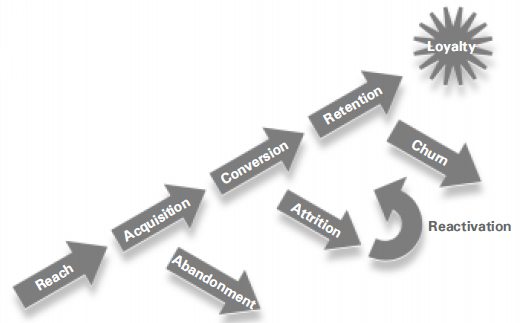
\includegraphics[width=1\textwidth]{lifecycle}
    \caption{Customer lifecycle \cite{Sterne2000}}
    \label{fig:lifecycle}
  \end{center}
\end{figure}

It starts by reaching the target audience or market up to an established 
customer base, not forgetting about those that drop mid way, due to abandonment 
or attrition.

\begin{itemize}
    \item \textbf{Reach} happens outside of the website and refers to the 
    number of potential customers. For example, if the online store is 
    advertised on a social network, the reach is the number of users who were 
    served the ad in that other website, they may or may not ignore it.
    \item \textbf{Acquisition} is the next stage, where the user decides to act 
    on and visits the website (or some other action like subscribing to a 
    newsletter).
    \item \textbf{Conversion} is the stage where a visitor stops being a user 
    and starts being a customer. It usually means that the user made a purchase 
    but some companies might consider a sign up or registration in the website 
    as a conversion.
    \item \textbf{Retention} focuses on making existing customers, that made at 
    least  one purchase before, repeat purchases.
    \item \textbf{Loyalty} is a stronger form of retention, which represents a 
    greater trust level of the customer in the store.
    \item \textbf{Abandonment} is defined by the customers that started the 
    buying process but do not finish it. For example, a customer may add items 
    to the online shopping cart but instead of moving to the next step, e.g. 
    enter credit card details, they exit the website or go elsewhere. This may 
    happen in any store with a multi-step buying process, which is very common.
    \item \textbf{Attrition} happens when a retained customer ceases buying 
    from the store and starts using a competitor store.
    \item \textbf{Churn} is defined by the number of customers that attrited 
    during a certain period divided by the total number of customers at the end 
    of that period. It measures how much of the customer base "rolls over" in a 
    certain time period.
\end{itemize}

\section{Customer Behaviour Model Graph (CBMG)}

A state transition graph named Customer Behaviour Model Graph (CBMG) can be 
used to describe the behaviour of customers browsing a website. The nodes 
represent the possible states or pages, e.g home page, product page, search, 
and a probability is associated with each transition. An example of such a CBMG 
is shown in figure \ref{fig:cbmg}.

\begin{figure}[h]
    \begin{center}
        \leavevmode
        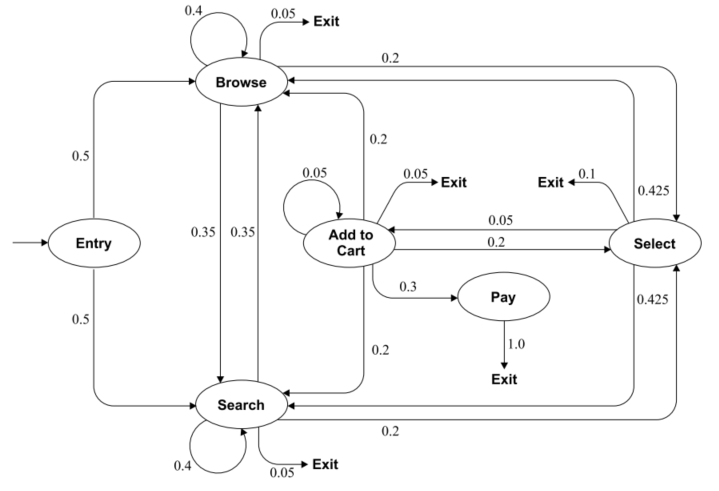
\includegraphics[width=1\textwidth]{cbmg}
        \caption{Example of a customer behaviour model graph \cite{Menasce1999}}
        \label{fig:cbmg}
    \end{center}
\end{figure}

\cite{Menasce1999} describes how CBMGs can be used to analyse the workload of 
an e-commerce store server and how metrics can be derived directly from the 
CBMG alone.

\section{E-commerce metrics}

Metrics are a common way to quantify, measure, benchmark or evaluate some 
process. In an e-commerce setting, businesses are interested in optimizing, 
mostly, for profit. Different businesses prioritize metrics in different ways, 
adapted to each use case. Here we present some commonly used metrics, but this 
list is by no means exhaustive. \cite{Sterne2000, Menasce1999}

% \todo{cyber report metrics}

\begin{itemize}
    \item \textit{Conversion Rate} (CR) is the percentage of visitors that buy 
    a product or a service;
    \item \textit{Shopping Cart Abandonment} is the percentage of visitors that 
    added a product to the online cart but did not complete the process;
    \item \textit{Average Order Value} (AOV) is the average cost of all orders;
    \item \textit{Customer Lifetime Value} (LTV) is the projected value that a 
    customer will spend on the store;
    \item \textit{Clicks to Buy} (CTB) is the average number of clicks a 
    visitor has to do to complete a buy order;
    \item \textit{Churn Rate} the percentage of customers that do not make a 
    repeated purchase;
    \item \textit{Bounce Rate} is the percentage of visitors that arrive at the 
    homepage of the online store but leave immediately, without clicking 
    anything or visiting a different page.
\end{itemize}

There are other common metrics such as \textit{Acquisition Cost}, \textit{Cost 
Per Conversion}, \textit{Net Yield} or \textit{Connection Rate} however they 
are associated with promotion campaigns that happen outside of the store 
website, therefore they are not interesting in the context of our work.

\section{Influencing user behaviour}

\cite{Constantinides2004} describes functionality, psychological and content 
factors that can influence the visitor experience, represented in the table 
\ref{tab:factors}.

\begin{table}[h]
    \centering
    \caption{Main building blocks of Web experience and their sub-categories 
    \cite{Constantinides2004}}
    \label{tab:factors}
    \begin{tabular}{@{}lll@{}}
\toprule
\multicolumn{2}{c}{\textbf{Functionality factors}} & \textbf{} \\ \midrule
\textbf{Usability} & \textbf{Interactivity} & \textbf{} \\ \midrule
Convenience & Customer &  \\
Site navigation & Interaction with company personnel &  \\
Information architecture & Customization &  \\
Ordering/payment process & Network effects &  \\
Search facilities and process &  &  \\
Site speed &  &  \\
Findability/accessibility &  &  \\ \midrule
\multicolumn{1}{c}{\textbf{Psychological factors}} & 
\multicolumn{2}{c}{\textbf{Content factors}} 
\\ \midrule
\textbf{Trust} & \textbf{Aesthetics} & \textbf{Marketing mix} \\ \midrule
Transaction security & Design & Communication \\
Customer data misuse & Presentation quality & Product \\
Customer data safety & Design elements & Fulfillment \\
Uncertainty reducing elements & Style/atmosphere & Price \\
Guarantees/return policies &  & Promotion \\
&  & Characteristics \\ \bottomrule
    \end{tabular}
\end{table}

Regarding usability of the online store, providing a personalized experience to 
each customer can be very beneficial for both the customer and the business. A 
common way to do this is by recommending products that the customer might be 
interested in~\cite{Adomavicius2005}. For example, if we know that a customer 
buys mostly football related products, recommending her more products in the 
same category might increase sales.

\section{Summary}

In this chapter we covered a brief overview of e-commerce, starting with the 
customer lifecycle, how to measure it using metrics and presenting a common way 
to model the users' behaviour, the CBMG.
